\documentclass[ngerman,a4paper,order=firstname]{../../texmf/tex/latex/mathscript/mathscript}
\usepackage{../../texmf/tex/latex/mathoperators/mathoperators}

\title{\textbf{Programmieren für Mathematiker WS2017/18}}
\author{Dozent: Prof. Dr. Wolfgang Walter}

\begin{document}
\pagenumbering{roman}
\pagestyle{plain}

\maketitle

\hypertarget{tocpage}{}
\tableofcontents
\bookmark[dest=tocpage,level=1]{Inhaltsverzeichnis}

\pagebreak
\pagenumbering{arabic}
\pagestyle{fancy}

\chapter*{Vorwort}
Schön, dass du unser Skript für die Vorlesung \textit{Lineare Algebra und analytische Geometrie 1} bei Prof. Dr. Arno Fehm im WS2017/18 gefunden hast! \footnote{Obwohl man sagen kann, dass es in dieser Vorlesung nur um Lineare Algebra ging, der Teil mit der analytischen Geometrie wurde vernachlässigt. Liegt wahrscheinlich auch daran, dass es demnächst eine Reform der Studienordnung gibt, in der aus der Vorlesung \textit{Lineare Algebra und analytische Geometrie} die Vorlesung \textit{Einführung in die Lineare Algebra} wird.}

Wir verwalten dieses Skript mittels Github \footnote{Github ist eine Seite, mit der man Quelltext online verwalten kann. Dies ist dahingehend ganz nützlich, dass man die Quelltext-Dateien relativ einfach miteinander synchronisieren kann, wenn man mit mehren Leuten an einem Projekt arbeitet.}, d.h. du findest den gesamten \LaTeX-Quelltext auf \url{https://github.com/henrydatei/TUD_MATH_BA}. Unser Ziel ist, für alle Pflichtveranstaltungen von \textit{Mathematik-Bachelor} ein gut lesbares Skript anzubieten. Für die Programme, die in den Übungen zur Vorlesung \textit{Programmieren für Mathematiker} geschrieben werden sollen, habe ich ein eigenes Repository eingerichtet; es findet sich bei \url{https://github.com/henrydatei/TU_PROG}.

Du kannst dir gerne dort die \LaTeX-Quelldateien herunterladen, die Dateien für exakt dieses Skript sind im Ordner \texttt{1. Semester/LAAG ueberarbeitet}. Es lohnt sich auf jeden Fall während des Studiums die Skriptsprache \LaTeX{} zu lernen, denn Dokumente, die viele mathematische oder physikalische Formeln enthalten, lassen sich sehr gut mittels \LaTeX{} darstellen, in Word oder anderen Office-Programmen sieht so etwas dann eher dürftig aus.

\LaTeX{} zu lernen ist gar nicht so schwierig, ich habe dafür am Anfang des ersten Semesters wenige Wochen benötigt, dann kannte ich die wichtigsten Befehle und konnte den Vorgänger dieses Skriptes schreiben (\texttt{1. Semester/LAAG}, Vorsicht: hässlich, aber der Quelltext ist relativ gut verständlich).

Es sei an dieser Stelle darauf hingewiesen (wie in jedem anderem Skript auch \smiley{}), dass dieses Skript nicht den Besuch der Vorlesungen ersetzen kann. Es könnte sein, dass Prof. Fehm seine Vorlesung immer mal wieder an die Studenten anpasst; wahrscheinlich immer dann, wenn die Prüfungsergebnisse zu schlecht waren. Nichtsdestotrotz veröffentlicht Prof. Fehm sein Skript auf seiner Homepage \url{http://www.math.tu-dresden.de/~afehm/lehre.html}. Allerdings ist dieses Skript recht hässlich, besonders was die Übersichtlichkeit angeht.

Wir möchten deswegen ein Skript bereitstellen, dass zum einen übersichtlich ist, zum anderen \textit{alle} Inhalt aus der Vorlesung enthält, das sind insbesondere Diagramme, die sich nicht im offiziellen Skript befinden, aber das Verständnis des Inhalts deutlich erleichtern. Ich denke, dass uns dies erfolgreich gelungen ist.

Trotz intensivem Korrekturlesen können sich immer noch Fehler in diesem Skript befinden. Es wäre deswegen ganz toll von dir, wenn du auf unserer Github-Seite \url{https://github.com/henrydatei/TUD_MATH_BA} ein neues Issue erstellst und damit auch anderen hilfst, dass dieses Skript immer besser wird.

\chapter{allgemeine Informationen}
\section{Allgemeines über Pointer}

Pointer nennt man auch \begriff{Zeiger}, \begriff{Verweise} oder \begriff{Datenreferenzen}. Ein Pointer ist ein Verweis bzw. eine Referenz auf ein Zielobjekt/Zeigerziel/Target eines festgelegten Datentyps. In den folgenden Darstellungen ist:
\begin{center}
	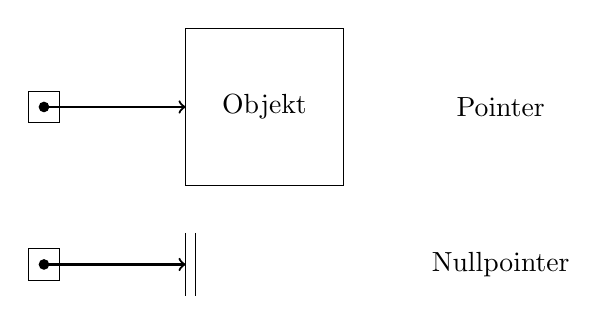
\begin{tikzpicture}[scale=0.2]
		\draw (0,0) -- (2,0);
		\draw (0,0) -- (0,2);
		\draw (2,0) -- (2,2);
		\draw (0,2) -- (2,2);
		\draw[fill = black] (1,1) circle (0.3);
		\draw[->, thick] (1,1) -- (10,1);
		\draw (10,-4) -- (10,6);
		\draw (10,-4) -- (20,-4);
		\draw (10,6) -- (20,6);
		\draw (20,-4) -- (20,6);
		\node at (15,1) (n) {Objekt};
		\node at (30,1) (n2) {Pointer};
		
		\draw (0,-10) -- (2,-10);
		\draw (0,-10) -- (0,-8);
		\draw (2,-10) -- (2,-8);
		\draw (0,-8) -- (2,-8);
		\draw[fill = black] (1,-9) circle (0.3);
		\draw[->, thick] (1,-9) -- (10,-9);
		\draw (10,-7) -- (10,-11);
		\draw (10.6,-7) -- (10.6,-11);
		\node at (30,-9) (n2) {Nullpointer};
	\end{tikzpicture}
\end{center}

Ein Pointer hat zu Beginn der Programmausführung einen undefinierten Zustand, der nicht als solcher erkannt werden kann. Die Verwendung eines solchen Pointers kann große Probleme verursachen.

Zeiger sind kein eigenständiger Typ, sondern nur mit dem Attribut \texttt{pointer} gekennzeichnet:
\begin{lstlisting}
! eine normale Variable
integer :: variable
! ein Pointer
integer, pointer :: ptr
\end{lstlisting}

Zeiger sind streng typisiert, das heißt man kann nur auf Objekte zeigen, deren Typ identisch mit dem Zeigertyp ist. Es gibt also keine Universalpointer. Der Pointer im oberen Quelltext kann also nur auf Variablen mit dem Typ \texttt{integer} zeigen.

Jedes beliebige Objekt vom passenden Objekttyp kann als Ziel eines Zeigers dieses Typs verwendet werden, wenn die Zielvariable das Attribut \texttt{target} trägt oder das Objekt ein dynamisches im Heap erzeugtes Objekt ist.
\begin{lstlisting}
integer, target :: ziel
integer, pointer :: ptr
\end{lstlisting}

Jede Pointer-Variable kann als Zeigerziel dienen. Ohne \texttt{target}-Attribut.

Implizit werden Pointer immer automatisch dereferenziert, außer in den Anweisungen \texttt{nullify()}, \texttt{allocate()}, \texttt{deallocate()}, der Pointer-Zuweisung \texttt{pointer => ziel} sowie in der \texttt{associated}-Abfragefunktion.

Pointer sind in Fortran in der Regel mehr als nur Adressen.

Werfen wir nun nochmal einen Blick auf die Pointer-Kontexte, in denen Pointer automatisch dereferenziert werden.

\begin{*anmerkung}
	Wird gerne in der Klausur abgefragt, steht aber auch in dem zur Klausur zugelassenen Buch des Rechenzentrums Niedersachsen über den Fortran-Standard.
\end{*anmerkung}

\begin{itemize}
	\item Die Funktion \texttt{nullify(p1, p2, ...)} versetzt die Pointer \texttt{p1}, \texttt{p2} und so weiter in den definierten Zustand Null = nicht assoziiert.
	\item \texttt{allocate(p1, p2, ...)} legt Speicherblöcke im Heap für die Zielobjekte der Pointer an und setzt die Pointer als Referenzen auf ihren jeweiligen Speicherblock. Alle Pointer sind im definierten Zustand assoziiert.
	\item Mit \texttt{deallocate(p1, p2, ...)} werden die Speicherblöcke, auf die die Pointer zeigen freigegeben und die Pointer auf Null gesetzt. Der Pointer muss dafür assoziiert und ein ganzen Objekt, also kein Subarray, Substring oder ähnliches, sein.
	\item Pointer werden mit \texttt{ptr => tgt} oder \texttt{ptr1 => ptr2} zugewiesen.
	\item Die Abfragefunktion \texttt{associated()} kann auf recht unterschiedliche Weisen eingesetzt werden:
	\begin{itemize}
		\item \texttt{associated(ptr)} $\to$ \texttt{.true.}, wenn auf ein Ziel gezeigt wird; \texttt{.false.}, wenn \texttt{ptr} auf Null zeigt.
		\item \texttt{associated(ptr, tgt)} $\to$ \texttt{.true.}, wenn \texttt{ptr} auf \texttt{tgt} zeigt, sonst \texttt{.false.}
		\item \texttt{associated(ptr1, ptr2)} $\to$ \texttt{.true.}, wenn beide Pointer denselben Zustand (nicht Null) haben, sonst \texttt{.false.}
	\end{itemize}
\end{itemize}

Wie schon oben angesprochen, ist der Umgang mit Pointern nicht ganz ungefährlich, es gibt einige Gefahren für den Hauptspeicher, insbesondere den Heap.

\begin{*anmerkung}
	auch wichtig in der Klausur, steht aber leider nicht im Buch, muss also auswendig gelernt werden
\end{*anmerkung}

\begin{itemize}
	\item Verwendung eines nicht definierten oder nicht gültigen Pointers in \texttt{deallocate}, \texttt{=>}, \texttt{associated}-Abfragen und normalen (nicht Pointer-) Kontext, das heißt in Expressions, in denen alle Pointer automatisch dereferenziert werden.
	\item \begriff{Dangling Pointer} entstehen, wenn das Zeigerziel verloren geht, z.B. durch \texttt{deallocate} über anderen Pointern oder eines \texttt{allocatable}-Feldes oder wenn das Zielobjekt "'out of scope"' geht, zum Beispiel durch Verlassen seiner Prozedur.
	\item \begriff{Speicherleichen}, Garbage, memory leaks: haben im Prinzip das ewige Leben im Heap, wenn keine Referenzen mehr auf ein Heap-Objekt existiert, über die man es freigeben könnte.
\end{itemize}

\chapter{Zahldarstellungen}
\section{Basis-Konvertierung ganzer Zahlen}

Die Notation $[9]_{10}$ bedeutet, dass man die Zahl 9 im Zehner-System betrachtet. Es gilt also $[9]_{10} = [1001]_2$ und $[10]_{10}=[1010]_2$. 

Um eine Zahl von einer gegebenen Basis in eine Zielbasis $b$ zu konvertieren, so teilt man immer wieder durch $b$ und notiert den Rest als nächste Ziffer von hinten nach vorne. Am Beispiel von $[57]_{10}$ ins Zweier-System sieht das so aus:
\begin{align}
	\frac{57}{2} &= 28\text{ Rest } 1 \Rightarrow\text{ letzte Ziffer der Binärdarstellung} \notag \\
	\frac{28}{2} &= 14\text{ Rest } 0 \Rightarrow\text{ vorletzte Ziffer der Binärdarstellung} \notag \\
	\frac{14}{2} &= 7\text{ Rest } 0 \notag \\
	\frac{7}{2} &= 3\text{ Rest } 1 \notag \\
	\frac{3}{2} &= 1\text{ Rest } 1 \notag \\
	\frac{1}{2} &= 0\text{ Rest } 1 \notag
\end{align}
Also gilt: $[57]_{10}=[111001]_2$.

Die umgekehrte Richtung verläuft ähnlich:
\begin{center}
	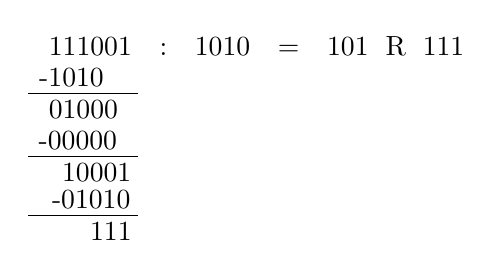
\begin{tikzpicture}
		\node at (0,0) (a) {111001\quad :\quad 1010\quad =\quad 101\; R\; 111};
		\node at (-2.35,-0.4) (b) {-1010};
		\draw (-2.9,-0.6) -- (-1.5,-0.6);
		\node at (-2.2, -0.8) (c) {01000};
		\node at (-2.27, -1.2) (d) {-00000};
		\draw (-2.9,-1.4) -- (-1.5,-1.4);
		\node at (-2.03,-1.6) (e) {10001};
		\node at (-2.1,-1.95) (f) {-01010};
		\draw (-2.9,-2.15) -- (-1.5,-2.15);
		\node at (-1.85,-2.35) (g) {111};
	\end{tikzpicture}
\end{center}
Also $[111001]_2$ durch $[10]_{10}=[1010]_2$ gleich $[101\text{ Rest }111]_2=[5\text{ Rest }7]_{10}\Rightarrow [57]_{10}$.

Von Basis 2 in Basis 4, 8 oder 16 ist dann ganz einfach: $[111100101]_2$
\begin{itemize}
	\item Zweiergruppen von hinten nach vorne zusammenzählen: $[13211]_4$
	\item Dreiergruppen von hinten nach vorne zusammenzählen: $[745]_8$
	\item Vierergruppen von hinten nach vorne zusammenzählen: $[1E5]_{16}$
\end{itemize}
\section{Basis-Konversion gebrochener Zahlen}

Festkommadarstellung (nur Betrag der Zahl, ohne Vorzeichen):
\begin{center}
	\begin{tabular}{rcccccccccc}
		Gewichte & $B^{k}$ & $B^{k-1}$ & ... & $B^1$ & $B^0$ & . & $B^{-1}$ & $B^{-2}$ & ... & $B^{-l}$ \\
		Ziffern & $m_k$ & $m_{k+1}$ & ... & $m_{-1}$ & $m_0$ & . & $m_{1}$ & $m_{2}$ & ... & $m_{l}$ \\
	\end{tabular}
\end{center}
Also: $\sum\limits_{i=k}^l m_i\cdot B^{-i}$.

Die Konvertierung des ganzzahligen Anteils vor dem "'."' läuft wie gehabt. Um den gebrochenen Anteil zu konvertieren, multipliziert man wiederholt mit der Zielbasis $b$ und nimmt den jeweiligen ganzzahligen Anteil als Nachkommaziffern (von links nach rechts). Mit dem gebrochenen Anteil macht man weiter. Wir wollen die Zahl $[0.625]_{10}$ ins Zweiersystem konvertieren:
\begin{align}
	0.625 \cdot 2 &= \textbf{1}.25 \notag \\
	0.25 \cdot 2 &= \textbf{0}.5 \notag \\
	0.5 \cdot 2 &= \textbf{1} \notag
\end{align}
Also gilt: $[0.625]_{10}=[0.101]_2$.

Wieder anders herum:
\begin{align}
	0.101 \cdot 1010 &= \textbf{110}.010 \notag \\
	0.010 \cdot 1010 &= \textbf{10}.100 \notag \\
	0.100 \cdot 1010 &= \textbf{101}.0 \notag
\end{align}
Also gilt $[0.101]_2 = [0.110|10|101]_2 = [0.625]_{10}$.

Jetzt wollen wir $[0.1]_{10}$ ins Zweiersystem konvertieren:
\begin{align}
	0.1 \cdot 2 &= \textbf{0}.2 \notag \\
	0.2 \cdot 2 &= \textbf{0}.4 \\
	0.4 \cdot 2 &= \textbf{0}.8 \notag \\
	0.8 \cdot 2 &= \textbf{1}.6 \notag \\
	0.6 \cdot 2 &= \textbf{1}.2 \notag \\
	0.2 \cdot 2 &= \textbf{0}.4
\end{align}
Wie man sieht, sind die Zeilen (1) und (2) gleich, das heißt, diese Konvertierung wird unendlich lange laufen. Also: $[0.1]_{10}=[0.0\overline{0011}]_2$. Aber es muss gelten: $[0.1]_{10}\cdot [10]_{10}=[1]_{10}$. Aber es stimmt: $[0.0\overline{0011}]_2\cdot [1010]_2=[0.\overline{1}]_2=[1]_2$.

Entsprechend gilt:
\begin{align}
	[0.2]_{10} &= [0.\overline{0011}]_2 \notag \\
	[0.3]_{10} &= [0.01\overline{0011}]_2 \notag \\
	[0.4]_{10} &= [0.011\overline{0011}]_2 \notag \\
	[0.5]_{10} &= [0.1]_2 \notag \\
	[0.6]_{10} &= [0.1\overline{0011}]_2 \notag \\
	[0.7]_{10} &= [0.1011\overline{0011}]_2 \notag \\
	[0.8]_{10} &= [0.11\overline{0011}]_2 \notag \\
	[0.9]_{10} &= [0.111\overline{0011}]_2 \notag
\end{align}

Problem: Rundungen schon bei $\frac{1}{10}\Rightarrow$ falsche Nachkommastellen. Die Lösung sind hier Gleitkommazahlen.
\section{Gleitkommazahlen}

Gleitkommazahlen werden auch Fließkommazahlen, Gleitpunktzahlen, Fließpunktzahlen oder floating-point-numbers genannt.

Das \begriff{Gleitkommaformat} $R=(b,l,\underline{e},\overline{e})$ besteht aus
\begin{itemize}
	\item einer Basis $b$
	\item einer Mantissenlänge $l$
	\item einem Exponentenbereich von $\underline{e}$ bis $\overline{e}$.
\end{itemize}

Eine \begriff{Gleitkommazahl} ist entweder 0 oder $x=(-1)^s\cdot m\cdot b^e$ mit
\begin{itemize}
	\item Vorzeichenbit $s\in \{0,1\}$
	\item Mantisse $m=[0.m_1m_2m_3...m_l]_b$ mit Mantissenziffern $m_i\in\{0,1,2,...,b-1\}$
	\item $e\in\{\underline{e},\underline{e}+1,\underline{e}+2,...,\overline{e}\}$
\end{itemize}

Schauen wir uns das Beispiel $R(2,3,-1,+2)$ an. Eine solche Zahl benötigt 1 bit für $s$, 2 bits für $e$ und 3 bits für $m$.
\begin{center}
	\begin{tabular}{l|cccccccc}
		$m=$\textbf{ 0.} & \textbf{111} & \textbf{110} & \textbf{101} & \textbf{100} & \textbf{011} & \textbf{010} & \textbf{001} & \textbf{000} \\
		\hline
		$e=-1$ & \textcolor{Green}{$\frac{7}{16}$} & \textcolor{Green}{$\frac{6}{16}$} & \textcolor{Green}{$\frac{5}{16}$} & \textcolor{Green}{$\frac{4}{16}$} & \textcolor{red}{$\frac{3}{16}$} & \textcolor{red}{$\frac{2}{16}$} & \textcolor{red}{$\frac{1}{16}$} & 0 \\
		$e=0$ & \textcolor{Green}{$\frac{14}{16}$} & \textcolor{Green}{$\frac{12}{16}$} & \textcolor{Green}{$\frac{10}{16}$} & \textcolor{Green}{$\frac{8}{16}$} & \textcolor{Cyan}{$\frac{6}{16}$} & \textcolor{Cyan}{$\frac{4}{16}$} & \textcolor{Cyan}{$\frac{2}{16}$} & \textcolor{Cyan}{0} \\
		$e=1$ & \textcolor{Green}{$\frac{28}{16}$} & \textcolor{Green}{$\frac{24}{16}$} & \textcolor{Green}{$\frac{20}{16}$} & \textcolor{Green}{$\frac{16}{16}$} & \textcolor{Cyan}{$\frac{12}{16}$} & \textcolor{Cyan}{$\frac{8}{16}$} & \textcolor{Cyan}{$\frac{4}{16}$} & \textcolor{Cyan}{0} \\
		$e=2$ & \textcolor{Green}{$\frac{56}{16}$} & \textcolor{Green}{$\frac{48}{16}$} & \textcolor{Green}{$\frac{40}{16}$} & \textcolor{Green}{$\frac{32}{16}$} & \textcolor{Cyan}{$\frac{24}{16}$} & \textcolor{Cyan}{$\frac{16}{16}$} & \textcolor{Cyan}{$\frac{8}{16}$} & \textcolor{Cyan}{0} \\
	\end{tabular}
\end{center}

Es gibt also auch mehrere Darstellungen für eine Zahl! Die \textcolor{Cyan}{Cyan} eingefärbten Zahlen können auch anders dargestellt werden. 

\textcolor{Green}{Grüne} Zahlen sind sogenannte \begriff[Gleitkommazahl!]{normalisierte Gleitkommazahlen}, ihre erste Mantissenziffer ist $\neq 0$. Die \textcolor{red}{roten} Zahlen sind \begriff[Gleitkommazahl!]{denormalisierte Gleitkommazahlen}: Ihre ersten Mantissenziffer ist $m_1=0$ und ihr Exponent $e=\underline{e}$. Da das erste Mantissenbit häufig eine 1 ist, wird angenommen, dass das erste Mantissenbit eine 1 ist und wird deswegen nicht gespeichert (hidden bit). Das sorgt dafür, dass bei 3 bit Genauigkeit mit 4 bit Genauigkeit gerechnet werden kann. Ist das erste Mantissenbit eine 0, gibt es dafür eine spezielle Exponentenkennung.

Ein Zahlenstrahl mit diesen Zahlen ist besonders dicht um 0, aber ab 2 werden die Abstände sehr groß.

Die größte darstellbare Zahl ist $x_{max}=0.1111...1=(1-b^l)\cdot b^{\overline{e}}$. \\
Der kleinste darstellbare normalisierte Betrag ist $x_{min,N} = 0.10000...0=b^{\underline{e}-1}$. \\
Der kleinste darstellbare denormalisierte Betrag ist $x_{min,D} = 0.0000...1=b^{\underline{e}-l}$.

Doch es gibt eine Probleme:
\begin{itemize}
	\item absolute/relative Fehler bei Zahlen, die zwischen 2 darstellbaren Zahlen liegen $\Rightarrow$ Rundungen bei nahezu jeder Rechnung!
	\item Grundrechenarten können nicht darstellbare Zahlen erzeugen
\end{itemize}
\section{Rundung}

Eine \begriff{Rundung} ist eine Funktion $O:\real\to\text{Gleitkomma-Raster }R$.

Eine Rundung $O$ hat folgende Eigenschaften:
\begin{enumerate}
	\item $O(x)=x$ wenn $x\in R$
	\item $x,y\in\real$ mit $x<y\Rightarrow O(x)<O(y)$
	\item \textcolor{Gray}{$O(-x)=-O(x)$, nur manche Rundungen haben diese Eigenschaft}
\end{enumerate}

Es gibt verschiedene Rundungsmodi:
\begin{itemize}
	\item "'to nearest"': zur nächsten Gleitkommazahl, wenn 2 Gleitkommazahlen gleich weit weg sind, wird abwechselnd auf- und abgerundet
	\item "'trancation"': Abschneiden der Nachkommastellen $\Rightarrow$ betragskleiner runden
	\item "'augmentation"': zusätzliche Stellen hinzufügen $\Rightarrow$ betragsgrößer runden
	\item "'upward"': nach oben runden
	\item "'downward"': nac unten runden
\end{itemize}

Wenn $O$ eine Rundung mit einem Rundungsmodus, also $O\in \{\text{Rundungsmodi}\}$, ist und $\circ$ eine Grundrechenart, also $\circ\in\{+,-,\cdot,\div\}$, dann gilt für eine Gleitkommaoperation $\odot$ 
\begin{align}
	x,y\in R: x\odot y := O(x\circ y)\notag
\end{align}

\textbf{Auslöschung} in Summen von Gleitkommazahlen tritt auf, wenn die Größenordnung der exakten Summe wesentlich kleiner ist als die Größenordnung der Summanden (bzw. der Zwischenergebnisse).

\chapter{Grundstrukturen von Algorithmen}
\section{Begriffe}

Eine \begriff{Sequenz} sind einzelne Anweisungen hintereinander. \\
Eine \begriff{Selektion} ist eine Verzweigung. \\
Eine \begriff{Repetition} ist eine Wiederholung.

\subsection{Variablen und Daten}

Wir sehen uns einen Biertrinker an, der nach dem Genuss noch ein paar Besorgungen machen muss. Dabei ergeben sich folgende Variablen
\begin{itemize}
	\item Variable \textbf{Durst} von Typ \textit{LOGICAL}
	\item Variable \textbf{Geld} von Typ \textit{INTEGER}
	\item Variable \textbf{PreisDerBesorgung} von Typ \textit{INTEGER}
	\item Variable \textbf{Rest} von Typ \textit{INTEGER}
	\item Variable \textbf{Bierpreis} von Typ \textit{INTEGER}
	\item Variable \textbf{WirtschaftAnnehmbar} von Typ \textit{LOGICAL}
	\item Variable \textbf{Autofahrer} von Typ \textit{LOGICAL}
	\item Variable \textbf{AlkoholGrenzwert} von Typ \textit{REAL}
	\item Variable \textbf{AlkoholVergiftungsWert} von Typ \textit{REAL}
\end{itemize}

\subsection{Schleifen}

In Fortran gibt es 4 Arten von \begriff{Schleifen}:
\begin{itemize}
	\item Endlosschleife
	\item Schleife mit Anfangsbedingung
	\item Schleife mit Endbedingung
	\item Zählschleife
\end{itemize}

Bei einer \begriff[Schleifen!]{Endlosschleife} wird der Anweisungsblock innerhalb der Schleife unendlich lange ausgeführt:
\begin{lstlisting}
do
 Anweisung1
 Anweisung2
 Anweisung3
end do
\end{lstlisting}

Bei einer \begriff[Schleifen!]{Schleife mit Anfangsbedingung} wird der Anweisungsblock nur ausgeführt, wenn die Anfangsbedingung wahr ist. Ist sie wahr, so wird der Block ausgeführt und anschließend überprüft, ob die Anfangsbedingung wieder wahr ist. Ist die Anfangsbedingung nicht wahr, so wird die Schleife nicht ausgeführt.
\begin{lstlisting}
do while(Anfangsbedingung)
 Anweisung1
 Anweisung2
 Anweisung3
end do
\end{lstlisting}

Hat die \begriff[Schleifen!]{Schleife eine Endbedingung}, so wird der Anweisungsblock auf jedem Fall 1-mal ausgeführt. Erst dann wird überprüft, ob die Endbedingung wahr ist. Ist sie das, wird die Schleife \textbf{verlassen}. Ist sie falsch, so wird die Schleife erneut ausgeführt.
\begin{lstlisting}
do
 Anweisung1
 Anweisung2
 Anweisung3
 if(Endbedingung) exit
end do
\end{lstlisting}

Eine \begriff[Schleifen!]{Zählschleife} in Fortran ist ähnlich wie in anderen Programmiersprachen konzipiert, aber die Syntax ist deutlich verschieden. Eine Zählschleife besitzt eine Zählvariable (die auch in der Schleife benutzt werden kann, aber nicht geändert werden sollte), die von einer Anfangszahl mit bestimmter Schrittweite solange hochgezählt (oder bei negativer Schrittweite heruntergezählt) wird, bis die Zählvariable die Endzahl erreicht.
\begin{lstlisting}
do i = anfang, ende, schrittweite
 Anweisung1
 Anweisung2
 Anweisung3
end do
\end{lstlisting}

Bitte beachten:
\begin{itemize}
	\item Der Zustand der Zählvariable \texttt{i} vor der Schleife geht verloren, auch wenn die Schleife 0-mal läuft.
	\item Die Zählvariable \texttt{i} darf im Inneren der Schleife nicht geändert werden.
	\item Der Endzustand der Zählvariable \texttt{i} ist nach der Schleife nicht definiert.
	\item Ausdrücke werden zu Beginn genau 1-mal (vor der ersten Iteration) berechnet und sind dann fest.
	\item Die Anzahl der Iterationen ist: $N=\max\left\lbrace 0,\texttt{nint}\left(\frac{\texttt{ende }-\texttt{ anfang }+\texttt{ i}}{\texttt{i}}\right)\right\rbrace$
\end{itemize}

\section{Einfache Syntax}

Es gibt einen zulässigen Fortran-Zeichensatz. Dieser umfasst zum Beispiel die Buchstaben A-Z und a-z, sowie 0-9, Sonderzeichen und Operatoren.

Nun einige lexikalische Einheiten (Symbole/Tokens):
\begin{itemize}
	\item Keywords sind nicht reserviert, Variablen können also auch nach Keywords benannt werden.
	\item Identifiers (Namen) haben eine Länge von maximal 63 Zeichen. Variablen können Buchstaben, Zahlen und auch den Unterstrich enthalten.
	\item Literale (Konstanten): 3 $\Rightarrow$ INTEGER, 2.876 $\Rightarrow$ REAL, .TRUE. $\Rightarrow$ LOGICAL, "'Hallo"' $\Rightarrow$ STRING
	\item Labels (Marken): 00000 ... 99999 sind Sprungmarken, die mit \texttt{GOTO 99999} erreicht werden können.
	\item Separatoren (Trennsymbole) sind: \texttt{()}, \texttt{/}, \texttt{/(/)}, \texttt{[]}, \texttt{=}, \texttt{=>}, \texttt{:}, \texttt{::}, \texttt{,}, \texttt{;} und \texttt{\%}.
	\item Operatoren sind: \texttt{+}, \texttt{-}, \texttt{*},\texttt{/}, \texttt{**}, \texttt{//}, \texttt{==}, \texttt{<=}, \texttt{<}, \texttt{/=}, \texttt{>}, \texttt{>=}, \texttt{.NOT.}, \texttt{.OR.}, \texttt{.AND.}, \texttt{.EQV.} und \texttt{.NEQV.}.
\end{itemize}

In den alten Quellformen bis vor Fortran-90, also insbesondere Fortran-66 und Fortran-77 waren
\begin{itemize}
	\item Namen maximal 6 Zeichen lang und
	\item Lochkarten 80 Zeichen breit.
\end{itemize}

\begin{center}
	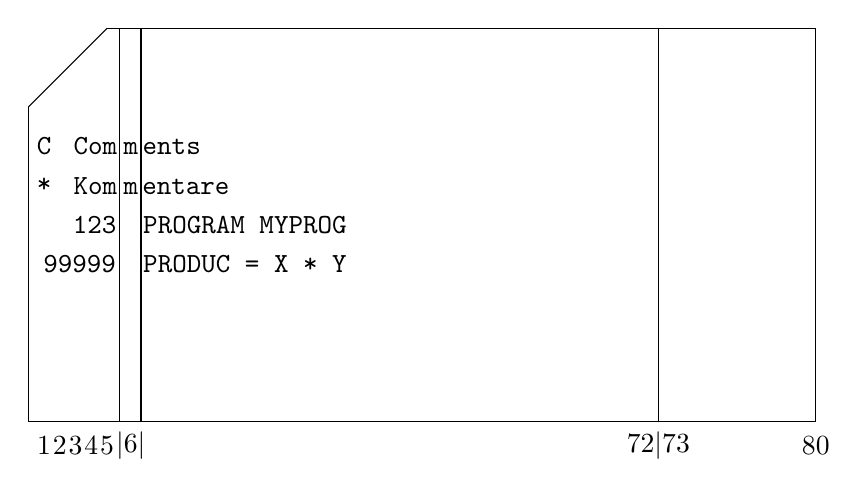
\begin{tikzpicture}
		\draw (0,0) -- (10,0);
		\draw (0,0) -- (0,4);
		\draw (0,4) -- (1,5);
		\draw (1,5) -- (10,5);
		\draw (10,0) -- (10,5);
		
		\node at (10,-0.3) (ende) {80};
		\node at (8,-0.3) (mitte) {$72\vert73$};
		\node at (0.2,-0.3) (1) {1};
		\node at (0.4,-0.3) (2) {2};
		\node at (0.6,-0.3) (3) {3};
		\node at (0.8,-0.3) (4) {4};
		\node at (1,-0.3) (5) {5};
		\node at (1.3,-0.3) (6) {$\vert 6\vert$};
		
		\draw (1.16,0) -- (1.16,5);
		\draw (1.43,0) -- (1.43,5);
		\draw (8,0) -- (8,5);
		
		\node at (0.2,3.5) (c) {\texttt{C}};
		\node at (0.85,3.5) (Com) {\texttt{Com}};
		\node at (1.3,3.47) (m) {\texttt{m}};
		\node at (1.82,3.488) (ents) {\texttt{ents}};
		
		\node at (0.2,3) (stern) {\texttt{*}};
		\node at (0.85,3) (Kom) {\texttt{Kom}};
		\node at (1.3,2.97) (m2) {\texttt{m}};
		\node at (2,2.99) (entare) {\texttt{entare}};
		
		\node at (0.84,2.5) (123) {\texttt{123}};
		\node at (2.75,2.5) (myprog) {\texttt{PROGRAM MYPROG}};
		\node at (0.65,2) (99999) {\texttt{99999}};
		\node at (2.75,2) (product) {\texttt{PRODUC = X * Y}};
	\end{tikzpicture}
\end{center}

Ab Fortran-90 wurden neue Quellformen entwickelt, das heißt:
\begin{itemize}
	\item Zeilen sind nun maximal 132 Zeichen lang
	\item Kommentare beginnen mit "'!"' und gehen bis zum Zeilenende
	\item Eine neue Zeile ist eine neue Anweisung, außer die letzte Zeile endet mit "'\&"'
	\item "'\&"' am Zeilenende bedeutet, dass die nächste nicht-Kommentar und nicht-Leerezeile die Anweisung fortsetzt.
	\item Die Fortsetzung darf mit "'\&"' beginnen.
	\item Es sind maximal 39 Fortsaetzungszeilen möglich
	\item Leerzeichen sind signifkant $\Rightarrow$ alle lexikalischen Tokens sind am Stück zu schreiben.
	\item Groß- und Kleinschreibung ist nicht signifikant in Namen und Keywords
\end{itemize}
\section{Datentypen}

Fortran besitzt 5 Datentypen. Für jeden Datentyp gibt es spezielle dazugehörige Funktionen:
\begin{itemize}
	\item \textbf{Integer} für ganze Zahlen
	\item \textbf{Real} für reelle Zahlen
	\item \textbf{Complex} für komplexe Zahlen
	\item \textbf{Logical} für logische Werte
	\item \textbf{Character} für Strings
\end{itemize}

\subsection{Der Datentyp \texttt{Integer}}
	\begin{tabular}{l|l}
		mögliche Argumente & \texttt{integer(kind=...)} \\
		\hline
		Darstellung & $\{\langle Z\rangle\}$ \\
		\hline
		Wert & mindestens 1 Ziffer, höchstens unendlich \\
		\hline
		Wertemenge & normalerweise im 2er-Komplement: $\left[ -2^{l-1},2^{l-1}-1 \right]$ \\
		\hline
		Operationen & \texttt{+}, \texttt{-}, \texttt{*}, \texttt{/} (schneidet Nachkommastellen ab), \texttt{**} (schneidet Nachkommastellen ab)
	\end{tabular}

\textbf{Wichtige Funktionen:}
\begin{itemize}
	\item\texttt{sign(x,y)} gibt den Betrag von $x$, wenn $y\ge 0$ und $-\vert x\vert$, wenn $y<0$
	\item\texttt{int(x)} schneidet die Nachkommastellen von $x$ ab
	\item\texttt{floor(x)} rundet ab ($\lfloor x\rfloor$)
	\item\texttt{ceiling(x)} rundet auf ($\lceil x\rceil$)
	\item\texttt{selected\_int\_kind(k)} liefert KIND-Parameter des kleinsten INTEGER-Typs, der dem alle Zahlen mit $k$ Stellen darstellen kann
\end{itemize}

\subsection{Der Datentyp \texttt{Real}}
	\begin{tabular}{l|l}
		mögliche Argumente & \texttt{real(kind=...)} \\
		\hline
		Darstellung & $\{\langle Z\rangle\}.\{\langle Z\rangle\}E\pm\{\langle Z\rangle\}$ \\
		\hline
		Wert & mindestens 1 Ziffer, höchstens unendlich \\
		\hline
		Wertemenge &  \\
		\hline
		Operationen & \texttt{+}, \texttt{-}, \texttt{*}, \texttt{/}, \texttt{**}
	\end{tabular}

\textbf{Wichtige Funktionen:}
\begin{itemize}
	\item\texttt{aint(x)} schneidet die Nachkommastellen von $x$ ab
	\item\texttt{real(x)} konvertiert zu REAL
	\item\texttt{selected\_real\_kind(p,r)} liefert KIND-Parameter mit $p$ Ziffern in der Mantisse und $r$ Ziffern im Exponenten
\end{itemize}

\subsection{Der Datentyp \texttt{Complex}}
	\begin{tabular}{l|l}
		mögliche Argumente & \texttt{complex(kind=...)} \\
		\hline
		Darstellung & $(\langle\Re\rangle,\langle\Im\rangle)$ \\
		\hline
		Wert &$\Re$,$\Im$ vorzeichenbehaftete realle Konstanten \\
		\hline
		Wertemenge &  \\
		\hline
		Operationen & \texttt{+}, \texttt{-}, \texttt{*}, \texttt{/}, \texttt{**}
	\end{tabular}

\textbf{Wichtige Funktionen:}
\begin{itemize}
	\item\texttt{abs(c)} liefert den Betrag von $c$, also $\sqrt{x^2+y^2}$
	\item\texttt{real(c)} liefert den Realteil von $c$
	\item\texttt{aimag(c)} liefert den Imaginärteil von $c$
	\item\texttt{conj(c)} liefert das konjugiert Komplexe zu $c$
\end{itemize}

\subsection{Der Datentyp \texttt{Logical}}
	\begin{tabular}{l|l}
		mögliche Argumente & \\
		\hline
		Darstellung & \texttt{.TRUE.}, \texttt{.FALSE.} \\
		\hline
		Wert & \texttt{.TRUE.} oder \texttt{.FALSE.} \\
		\hline
		Wertemenge & {\texttt{.TRUE.},\texttt{.FALSE.}} \\
		\hline
		Operationen & \texttt{.AND.}, \texttt{.OR.}, \texttt{.NOT.}, \texttt{.EQV.}, \texttt{.NEQV}
	\end{tabular}

\subsection{Der Datentyp \texttt{Character}}
	\begin{tabular}{l|l}
		mögliche Argumente & \texttt{character(len=...)} \\
		\hline
		Darstellung & Zeichen \\
		\hline
		Wert & einzelnes Zeichen oder Zeichenketten \\
		\hline
		Wertemenge & alle möglichen Zeichenfolgen mit $l$ Zeichen \\
		\hline
		Operationen & \texttt{//} (Konkardination: fügt 2 Strings zusammen)
	\end{tabular}

\textbf{Wichtige Funktionen:}
\begin{itemize}
	\item\texttt{ichar(c)} gibt den internen ganzzahligen Zeichencode von $c$
	\item\texttt{char(i)} gibt den Zeichencode zu $c$
	\item $\langle\text{Zeichenkette}\rangle$\texttt{(a:b)} gibt den Teilstring vom $a$-ten bis zum $b$-ten Zeichen
	\item\texttt{len(zk)} gibt die Länge der Zeichenkette $zk$
	\item\texttt{trim(zk)} liefert die Zeichenkette ohne anhängende Leerzeichen
	\item\texttt{adjustl(zk)} Inhalt der Zeichenkette wird nach vorne geschoben
	\item\texttt{repeat(zk,copies)} gibt einen String mit $copies$-facher Zeichenkette
	\item\texttt{index, scan, verify} durchsucht einen String
\end{itemize}

Es gibt allerdings noch eine Reihe weiterer (mathematischer) Funktionen, das Ergebnis ist selbsterklärend:
\begin{itemize}
	\item\texttt{sin(x)}, \texttt{asin(x)}, \texttt{sinh(x)}
	\item\texttt{cos(x)}, \texttt{acos(x)}, \texttt{cosh(x)}
	\item\texttt{tan(x)}, \texttt{atan(x)}, \texttt{atan2(x,y)=atan(x/y)}
	\item\texttt{sqrt(x)}
	\item\texttt{exp(x)}
	\item\texttt{log10(x)}
\end{itemize}

\subsection{INTEGER-Division}

Die klassiche INTEGER-Division sieht so aus:
\begin{center}
	\begin{tabular}{ll}
		Division: & $\frac{a}{b} =$ \texttt{a/b} \\
		Rest der Division: & $a-\left(\frac{a}{b}\right)\cdot b =$ \texttt{mod(a,b)} \\
		\hline
		\textbf{Beispiele (Division)} & \textbf{Beispiele (Rest)} \\
		\hline
		$\frac{8}{5} \to 1$ & \texttt{mod(8,5)} $\to$ 3 \\
		$\frac{-8}{5} \to -1$ & \texttt{mod(-8,5)} $\to$ -3 \\
		$\frac{-8}{-5} \to 1$ & \texttt{mod(-8,-5)} $\to$ -3 \\
		$\frac{8}{-5} \to -1$ & \texttt{mod(8,-5)} $\to$ 3
	\end{tabular}
\end{center}

Das darf man aber nicht mit der nach unten abgerundeten REAL-Division verwechseln:
\begin{center}
	\begin{tabular}{ll}
		Division: & $\left\lfloor\frac{a}{b}\right\rfloor =$ \texttt{floor(a/b)} = \texttt{floor(real(a)/real(b))} \\
		Rest der Division: & $a-\left\lfloor\frac{a}{b}\right\rfloor\cdot b =$ \texttt{modulo(a,b)} \\
		\hline
		\textbf{Beispiele (Division)} & \textbf{Beispiele (Rest)} \\
		\hline
		$\frac{8.0}{5.0} \to 1$ & \texttt{modulo(8,5)} $\to$ 3 \\
		$\frac{-8.0}{5.0} \to -2$ & \texttt{modulo(-8,5)} $\to$ 2 \\
		$\frac{-8.0}{-5.0} \to 1$ & \texttt{modulo(-8,-5)} $\to$ -3 \\
		$\frac{8.0}{-5.0} \to -2$ & \texttt{modulo(8,-5)} $\to$ -2
	\end{tabular}
\end{center}

\subsection{Potenzieren}

Die Potenz-Operation \texttt{**} ist die einzige Operation die von rechts nach links gelesen wird, bei allen anderen Operationen wird in Leserichtung, also von links nach rechts gearbeitet.
\begin{itemize}
	\item\texttt{2**3} $=2^3=8$
	\item\texttt{2**(-3)} $\to$ \texttt{int($2^{-3}$)=int($\frac{1}{8}$)} $=0$
	\item\texttt{(-3)**2} $=(-3)^2=9$
	\item\texttt{-3**2} $=-3^2=-9$
	\item\texttt{2**3**2} $=$ \texttt{2**(3**2)} $=2^9=512$
	\item\texttt{(2**3)**2} $=(2^3)^2=64$
\end{itemize}

\subsection{Operator-Prioritäten}

Operatoren haben in Fortran eine Priorität, die weiter gefasst ist als: "'Punktrechnung vor Strichrechnung"'. Operatoren mit der höchsten Priorität (12) werden zuerst ausgeführt; Operatoren mit der Priorität 1 zuletzt.
\begin{enumerate}
	\item selbstdefinierte Operatoren binär
	\item\texttt{.EQV.} und \texttt{.NEQV.}
	\item\texttt{.OR.}
	\item\texttt{.AND.}
	\item\texttt{.NOT.}
	\item Vergleichsoperatoren
	\item\texttt{//}
	\item\texttt{+}, \texttt{-} als Addition beziehungsweise Subtraktion
	\item\texttt{+}, \texttt{-} als Vorzeichen
	\item\texttt{*}, \texttt{/}
	\item\texttt{**}
	\item selbstdefinierte Operatoren unär
\end{enumerate}

Jetzt noch ein kurzer Abschnitt zu Variablen in imperativen Programmiersprachen. Eine Variable wird durch ein 5-Tupel (N,T,G,L,R) beschrieben, das heißt
\begin{itemize}
	\item N - Name
	\item T - Typ
	\item G - Gültigkeitsbereich
	\item L - l-Value (Zugriff auf die Variable)
	\item R - r-Value (Wert der Variable)
\end{itemize}

\section{Ausdrücke}

\begin{*anmerkung}
	Beliebtes Klausuren-Thema!
\end{*anmerkung}

Ein Ausdruck (= expression) wird in Fortran folgendermaßen ausgewertet:
\begin{enumerate}
	\item Konstanten und Objekte werden ausgewertet
	\item geklammerte Ausdrücke werden von innen nach außen ausgewertet
	\item Funktionen werden aufgerufen
	\item Operatoren höherer Priorität werden vor Operatoren niedrigerer Priorität behandelt
	\item sind die Prioritäten gleich, so wird von links nach rechts gearbeitet (Ausnahme: \texttt{**})
\end{enumerate}

Ein \begriff{Ausdrucksbaum} zeigt auf, wie in Fortran Ausdrücke ausgewertet werden: Für den Ausdruck (auch Infix-Notation)
\begin{align}
	\texttt{logo = i / j / x >= y .OR. - y / z < - x ** 3 ** 2 .AND. char <= 'p' // 'eter'}\notag
\end{align}
sieht der Baum folgendermaßen aus:
\begin{center}
	\begin{tikzpicture}[level/.style={sibling distance=60mm/#1}]
	\node[circle,draw] (root) {\texttt{.OR.}}
	child {node[circle,draw] (a) {\texttt{>=}}
		child {node[circle,draw] (b) {\texttt{/}}
			child {node[circle,draw] (c) {\texttt{/}}
				child {node[] (d) {$i$}}
				child {node[] (e) {$j$}}}
			child {node[] (f) {$x$}}}
		child {node[] (g) {$y$}}}
	child {node[circle,draw] (h) {\texttt{.AND.}}
		child {node[circle,draw] (i) {\texttt{<}}
			child {node[circle,draw] (j) {\texttt{-}}
				child {node[circle,draw] (k) {\texttt{/}}
					child {node[] (l) {$y$}}
					child {node[] (m) {$z$}}}}
			child {node[circle,draw] (q) {\texttt{-}}
				child {node[circle,draw] (p) {\texttt{**}}
					child {node[] (n) {$x$}}
					child {node[circle,draw] (o) {\texttt{**}}
						child {node[] (w) {3}}
						child {node[] (x) {2}}}}}}
		child {node[circle,draw] (r) {\texttt{<=}}
			child {node[] (s) {$char$}}
			child {node[circle,draw] (t) {\texttt{//}}
				child {node[] (u) {'p'}}
				child {node[] (v) {'eter'}}}}};
	\end{tikzpicture}
\end{center}

Es gibt verschiedene Notationen um Ausdrücke aufzuschreiben:
\begin{itemize}
	\item \begriff{Präfix-Notation}: Task $\to$ rekursiv linke Seite $\to$ rekursiv rechte Seite
	\item \begriff{Infix-Notation}: rekursiv linke Seite $\to$ Task $\to$ rekursiv rechte Seite
	\item \begriff{Postfix-Notation}: rekursiv linke Seite $\to$ rekursiv rechte Seite $\to$ Task
\end{itemize}

Für unseren Ausdruck bedeutet das:
\begin{itemize}
	\item Präfix-Notation: \texttt{= logo .OR. >= / / i j x y .AND. < NEG / y z NEG ** x ** 3 2 <= char // ‚p‘ ‚eter‘}
	\item Postfix-Notation: \texttt{logo i j / x / y >= y z / NEG x 3 2 ** ** NEG < char ‚p‘ ‚eter‘ // <= .AND. .OR. =}
\end{itemize}
\section{Unterprogramme}

In Fortran gibt es 2 Arten von Unterprogrammen: Funktionen und Subroutinen. \begriff{Funktionen} berechnen aus übergebenen Argumenten einen neuen Wert, während \begriff{Subroutinen} auch Anweisungen wie \texttt{write(*,*)} ausführen können. Eine Funktion sieht in Fortran folgendermaßen aus:
\begin{lstlisting}
function funcName(x,y,z)
 Anweisung1
 Anweisung2
 Anweisung3
end function funcName
\end{lstlisting}
Eine Subroutine so:
\begin{lstlisting}
subroutine subName(x,y,z)
 Anweisung1
 Anweisung2
 Anweisung3
end subroutine subName
\end{lstlisting}
Der Aufruf von Funktionen oder Subroutinen geht so:
\begin{lstlisting}
ergebnis = funcName(bla, bla, blub)
call subName(bla, bla, blub)
\end{lstlisting}

Die Variablen \texttt{x}, \texttt{y} und \texttt{z} sind sogenannte \begriff{formale Argumente}, die beim Aufruf des Unterprogramms im Hauptprogramm mit den \begriff{aktuellen Argumenten} \texttt{bla} und \texttt{blub} assoziiert werden. In vielen anderen Programmiersprachen (\textbf{Also nicht in Fortran!}) wird diese Assoziation als \begriff{call-by-value} realisiert, das heißt
\begin{itemize}
	\item Das aktuelle Argument wird ausgewertet und das Ergebnis wird in den korrekten Typ konvertiert.
	\item Der Ergebniswert wird als Initialwert an das formale Argument im Unterprogramm übergeben.
	\item Änderungen des formalen Arguments im Unterprogramm haben \textbf{keine} Auswirkungen auf das aktuelle Argument.
\end{itemize}
Fortran assoziiert hingegen mit \begriff{call-by-reference}, das heißt:
\begin{itemize}
	\item Das formale Argument wird für die gesamte Ausführungsdauer des Unterprogramms mit der Variable, die als aktuelles Argument übergeben wurde, assoziiert.
	\item Das heißt, dass das formale Argument ein Alias für die als aktuelles Argument übergebene Variable ist \\
	$\Rightarrow$ für die Dauer der Ausführung des Unterprogramms haben formales Argument und aktuelles Argument denselben l-Value \\
	$\Rightarrow$ Änderungen des formales Arguments bewirken die \textbf{gleichen} Änderungen des aktuelles Arguments.
\end{itemize}

In Fortran wird immer call-by-reference benutzt, allerdings darf das aktuelle aktuelle Argument auch ein Ausdruck sein, für dessen Ergebnis eine versteckte Variable angelegt wird, die per Referenz an das formale Argument übergeben wird. $\Rightarrow$ In diesem Fall sollen keine Änderungen am formalen Argument vorgenommen werden.

Unterprogramme werden in Fortran in 4 Schritten aufgerufen:
\begin{enumerate}
	\item Auswertung/Bestimmung des aktuellen Arguments
	\item Assoziation der aktuellen Argumente mit den formalen Argumente (per Referenz)
	\item Unterprogramm-Sprung
	\item Rücksprung an die Aufrufstelle bei erreichen einer \texttt{return}-Anweisung oder \texttt{end} im aufgerufenen Unterprogramm
\end{enumerate}

Da Fortran per call-by-reference assoziiert, gibt es verbotene Seiteneffekte (side effects). Diese dürfen \texttt{nicht} in Unterprogrammen verwendet werden.
\begin{itemize}
	\item Veränderungen von Variablen im Ausdruck durch Funktionsauswertung in demselben Ausdruck ($\Rightarrow$ die Auswertung ist abhängig von der Auswertungsreihenfolge) \\
	\texttt{Y = X + X * F(X)} $\to$ Zuerst werden alte \texttt{X} addiert, dann wird \texttt{X} modifiziert \\
	\texttt{Z = F(X) * X + X} $\to$ \texttt{X} wird verändert, dann werden neue \texttt{X} addiert. \\
	\texttt{if(x < f(x))} $\to$ besser wäre: \texttt{y = x; if(x < f(y))}
	\item Assoziation mehrerer formaler Argumente mit demselben aktuellen Argument, wenn eines dieser formalen Argumente innerhalb des Unterprogramms verändert wird:
	\begin{lstlisting}
subroutine sub(a,b)
 integer :: a, b
 b = a + b
end subroutine sub

call sub(x,x)
	\end{lstlisting}
\end{itemize}

Um solche Probleme zu vermeiden kann man formale Argumente mit einen Schreib- bzw. Leseschutz ausstatten. Dafür gibt es in Fortran das sogenannte \texttt{intent}-Attribut.
\begin{lstlisting}
subroutine test(a, input, output)
 integer, intent(inout) :: a
 integer, intent(in) :: input
 integer, intent(out) :: output
end subroutine test
\end{lstlisting}
\begin{itemize}
	\item \texttt{a} muss einen definierten Anfangszustand haben
	\item \texttt{input} hat einen Schreibschutz, es darf nur gelesen werden
	\item \texttt{output} hat einen Leseschutz, es darf nur geschrieben werden
\end{itemize}

Das \texttt{optional}-Attribut kann für formale Argumente benutzt werden, die nicht zwingend für die korrekte Funktionsweise des Unterprogramms notwendig sind. Im Unterprogramm muss man dann prüfen, ob dieses Argument übergeben wurde:
\begin{lstlisting}
subroutine sub(a,b,opt)
 integer :: a,b
 integer, optional :: opt
 
 if(present(opt))
  b = a + opt
 else
  b = a
 end if
end subroutine sub
\end{lstlisting}

Ein Unterprogramm kann sich auch selbst aufrufen, wenn das Unterprogramm das Attribut \texttt{recursive} besitzt. Diese sind charakterisiert durch: Mehrere Instanzen (Aktivierungen) des rekursiven Unterprogramms sind gleichzeitig aktiv, das heißt mehrere Instanzen seines Aktivierungsblocks können gleichzeitig auf dem Laufzeitstapel liegen. Im Aktivierungsblock liegen alle Parameter, lokalen Variablen, eventuell. ich andere Informationen zur Aufrufverwaltung (z.B. Rücksprungadresse, ...); jede Aktivierungsblockinstanz ist eine vollständige Kopie mit eigenem Speicher.
\begin{lstlisting}
recursive function fakultaet(n) result (res)
 integer, intent(in) :: n
 integer :: res
 
 if(n == 0) then
  res = 1
 else
  res = n * fakultaet(n-1)
 end if
end function fakultaet
\end{lstlisting}
\begin{lstlisting}
recursive function ggt(a,b) result (g)
 integer :: a, b, g
 
 if(b == 0) then
  g = a
 else
  g = ggt(b, mod(a,b))
 end if
end function ggt
\end{lstlisting}

Man kann viele Funktionen und Subroutinen auch in sogenannten \begriff{Modulen} zusammenfassen, die dann im Hauptprogramm mit \texttt{use modulname} eingebunden werden können. Beim Kompilieren ist darauf zu achten, dass immer von "'unten nach oben"' kompiliert wird, also vom untersten Modul bis zum Hauptprogramm.

Ein Modul definiert in der Regel einen ADT (abstrakter Datentyp), das heißt mindestens einen öffentlichen Datentyp samt aller notwendigen Grundoperationen auf/mit Objekten dieses Typs. Häufig wird die innere Struktur der Objekte (bzw. des Typs) vor Zugriffen von außen geschützt (Datenkapselung, information/data hiding, ...), um Fehler im Umgang mit diesen Objekten zu vermeiden (z.B. inkonsistente innere Zustände, ...).
\section{Benutzerdefinierte Typen}

In Modulen werden häufig Datentypen vom Benutzer definiert, zum Beispiel der Datentyp \texttt{kreis}
\begin{lstlisting}
type kreis
 private !kein Zugriff auf Komponenten im Hauptprogramm
 real :: radius
 real :: mitteX
 real :: mitteY
end type kreis
\end{lstlisting}

Für diesen neuen Datentyp funktionieren die alten Operatoren wie \texttt{+} nicht mehr (was soll den die Summe aus 2 Kreisen sein?). Deswegen muss man sich eine neue Addition von Kreisen ausdenken:
\begin{lstlisting}
function add(kreis1, kreis2)
 type(kreis), intent(in) :: kreis1, kreis2
 type(kreis) :: add
 
 add%raduis = kreis1%radius + kreis2%radius
 add%mitteX = (kreis1%mitteX + kreis2%mitteX) / 2
 add%mitteY = (kreis1%mitteY + kreis2%mitteY) / 2
end function add
\end{lstlisting}

Wie man sieht kann man mit \% auf die einzelnen Komponenten zugreifen. Um jetzt wirklich im Programm \texttt{kreis1 + kreis2} zu benutzen, muss man noch den Operator \texttt{+} überladen. Dazu werden generische Schnittstellen benutzt. Man kann auch das Gleichheitszeichen, also die Zuweisung \texttt{=} überladen.
\begin{lstlisting}
interface operator(+)
 module procedure add
end interface operator(+)

interface assignment(=)
 module procedure gleich
end interface assignment(=)
\end{lstlisting}

Diese Operatorüberladungen brauchen immer das \texttt{intent(in)}-Attribut in den Funktionen! Überladungen von \texttt{=} brauchen dagegen sowohl \texttt{inten(in)} als auch \texttt{intent(out)}.

Mit dem \texttt{interface}-Block kann man auch lange und sperrige Namen von Funktionen einkürzen, so dass man statt \texttt{langUndSperrig(a,b)} auch \texttt{kurz(a,b)} verwenden kann:
\begin{lstlisting}
interface kurz
 module procedure langUndSperrig
end interface kurz
\end{lstlisting}
\section{Felder (Arrays)}

Bisher hatten wir nur Skalare als Variablen. Was aber, wenn wir nicht wissen, wie viele Variablen wir brauchen werden. Dann helfen uns Felder. Felder haben eine homogene Datenstruktur, das heißt alle Elemente haben den selben Datentyp, den \begriff{Elementtyp}. Es gibt sowohl ein- als auch mehrdimensionale Felder (die höchste Dimension ist 15), also Vektoren, Matrizen, Tensoren, ... Der lesende als auch schreibende Zugriff erfolgt mittels ganzzahliger Indizees, also \texttt{vector(3)}, \texttt{matrix(2,5)}, \texttt{tensor(3,4,6)}, ... Unzulässige Indexwerte ermöglichen beliebige Speicherzugriffe auch außerhalb des Feldes, wenn sie nicht beim Kompilieren erkannt werden. Es kann also folgender Laufzeitfehler auftreten: \texttt{Index out of bounds}.

Der Feldtyp ist charakterisiert durch
\begin{itemize}
	\item den Elementtyp
	\item den Rang: Anzahl der Dimensionen
\end{itemize}

Die geometrische Gestalt (= shape) eines Feldes kann entweder statisch oder dynamisch definiert werden, und zwar durch Ausdehnungen in jeder einzelnen Dimension
\begin{lstlisting}
! eine 3x3 Matrix
integer, dimension(1:3, 1:3) :: matrix

! eine dynamsiche Matrix, deren Groesse spaeter 5x5 wird
integer, dimension(:,:), allocatable :: dynMatrix
allocate(dynMatrix(1:5, 1:5))
\end{lstlisting}

Eindimensionale Felder kann man in Fortran wie folgt füllen: (seit Fortran-03 kann man statt \texttt{(/ /)}) auch \texttt{[ ]} benutzen)
\begin{lstlisting}
(/1, 3, 5, 7, 9/) = (/(i, i=1,9,2)/) = (/(2*i+1, i=0,4)/)
\end{lstlisting}

Die Speicherreihenfolge ist in Fortran immer spaltenweise (colum-major), das heißt der erste Index läuft am schnellsten, der letzte Index am langsamsten. Will man dagegen zeilenweise einlesen und ausgeben, so behilft man sich eines kleinen Tricks:
\begin{lstlisting}
real, dimension(3,2) :: A
integer :: i

read(*,*) A ! liesst spaltenweise ein
read(*,*) (A(i:), i=1,3) ! liesst zeilenweise ein

do i=1, 3
 write(*,*) A(i:) ! gibt A zeilenweise aus
end do
\end{lstlisting}

Es gibt auch eine Menge vordefinierter Matrix-Funktionen
\begin{itemize}
	\item\texttt{size(A,i)}: Anzahl der Elemente in $i$-ter Dimension
	\item\texttt{lbound(A,i)}: kleinster Indexwert in $i$-ter Dimension
	\item\texttt{ubound(A,i)}: größter Indexwert in $i$-ter Dimension
	\item\texttt{size(A)}: $\sum_{i=1}^{r}$ \texttt{size(A,i)}: Gesamtzahl aller Elemente
	\item\texttt{shape(A)}: \texttt{(/size(A,1), size(A,2), ..., size(A,r)/)}
	\item\texttt{sum(A,1)}: Summation einzelner Spalten, Ergebnis ist ein Vektor
	\item\texttt{sum(A,2)}: Summation einzelner Zeilen, Ergebnis ist ein Vektor
	\item\texttt{sum(A)}: Summe aller Elemente
	\item\texttt{prod(A)}: Produkt aller Elemente
	\item\texttt{all(A == B)}: logisches UND, überprüft, ob beide Matrizen gleich sind (durch Vergleich der Einträge). Es können auch andere logische Verknüpfungen verwendet werden
	\item\texttt{any(A == B)}: logisches ODER, überprüft ob mindesten ein Element in beiden Matrizen (an der selben Stelle) gleich ist
	\item\texttt{transpose(A)}: transponiert Matrix
	\item\texttt{dot\_product(v,w)}: Skalarprodukt der Vektoren $v$ und $w$
	\item\texttt{matmul(A,B)}: Matrizenmultiplikation, geht auch mit einem Vektor
	\item\texttt{forall(i=1:n, k=1:m)}: spart doppelte \texttt{do}-Schleifen
\end{itemize}

\subsection{Subarrays (Teilfelder)}

Durch Angabe von Indexgrenzen kann man aus einem Feld einen Teil herausschneiden.
\begin{align}
	A = \begin{pmatrix}4&5&6&7&8\end{pmatrix} \quad\texttt{A(2:4)}\Rightarrow \begin{pmatrix}5&6&7\end{pmatrix} \notag \\
	B = \begin{pmatrix}1&2&3\\4&5&6\\7&8&9\end{pmatrix} \quad\texttt{B(1:2,2:3)}\Rightarrow \begin{pmatrix}4&5\\7&8\end{pmatrix} \notag
\end{align}

Man kann das ganze natürlich auch komplizierter machen: Sei $A$ ein Quader ($5\times 5\times 5$). Das Teilfeld \texttt{C = A(3,1:5:2,(/4,1,2/))} nimmt aus dem Quader die 3. Schicht und in dieser Matrix die 1., 3. und 5. Zeile mit der 4., 1. und 2. Zeile
\begin{align}
	C = \begin{pmatrix}
		\text{Speicherplatz 4} & \text{Speicherplatz 7} & \text{leer} & \text{Speicherplatz 1} & \text{leer}\\
		\text{leer} & \text{leer} & \text{leer} & \text{leer} & \text{leer}\\
		\text{Speicherplatz 5} & \text{Speicherplatz 8} & \text{leer} & \text{Speicherplatz 2} & \text{leer}\\
		\text{leer} & \text{leer} & \text{leer} & \text{leer} & \text{leer}\\
		\text{Speicherplatz 6} & \text{Speicherplatz 9} & \text{leer} & \text{Speicherplatz 3} & \text{leer}
	\end{pmatrix}\notag
\end{align}

Felder können auch formale Argumente sein, aber nur, wenn sie fester Gestalt sind oder als Felder übernommener Gestalt, welche durch die Gestalt des aktuellen Arguments durch die Parameterassoziation (per Referenz) festgelegt ist. Wenn Felder Funktionsergebnisse sein sollen, so müssen die Indexbereiche zum Aufrufzeitpunkt der Funktion berechnet werden können; Indexgrenzen können beliebige Integer-Ausdrücke sein, die von den Werten und Eigenschaften der aktuellen Argumente und globalen Variablen oder Konstanten abhängen.

\textbf{Wichtige Regel: } Keine \texttt{allocatable}-Felder als formale Argumente (sein Fortran-03 möglich), Feld-Ergebnis einer Funktion und als Typkomponenten.

\begin{lstlisting}
function fun(v,w)
 real,dimension(:), intent(in) :: v,w
 real,dimension(size(v),size(w)) :: fun
 integer :: i,k
 
 do i = 1, size(v)
  do k = 1, size(w)
   fun(i,k) = v(i) * w(k)
  end do
 end do
end function fun

function fun_effizient(v,w)
 real,dimension(:), intent(in) :: v,w
 real,dimension(size(v),size(w)) :: fun
 real,dimension(size(v),size(w)) :: A,B
 
 A = spread(source=v, dim=2, ncopies=size(w))
 B = spread(source=w, dim=1, ncopies=size(v)) 
 fun_effizient = A * B ! elementweise Multiplikation
end function fun_effizient
\end{lstlisting}

\subsection{\texttt{pure} Prozeduren}

\begin{*anmerkung}
	völlig unwichtig
\end{*anmerkung}

Ein Unterprogramm welches keine Seiteneffekte hat ist eine bloßes bzw. reines (pure) Unterprogramm. Ein Unterprogramm erzeugt dann keine Seiteneffekte, wenn es weder seine Eingabedaten, noch die Daten verändert, die außerhalb des Unterprogrammes liegen, es sei denn, es wären seine Ausgabedaten. In einem reinen Unterprogramm haben die lokalen Variablen keine \texttt{save}-Attribute, noch werden die lokalen Variablen in der Datendeklaration initialisiert.

Das \texttt{save}-Attribut ist bei Initialisierung von Variablen impliziert, d.h. eine Initialisierung in der Typdeklaration macht die Variable automatisch statisch (Lebensdauer = gesamte Programmlaufzeit).
\begin{lstlisting}
integer, save :: counter = 0
\end{lstlisting}

Reine Unterprogramme sind für das \texttt{forall}-Konstrukt notwendig: das \texttt{forall}-Konstrukt wurde für das parallele Rechnen konzipiert, weshalb hier der Computer entscheidet, wie das Konstrukt abgearbeitet werden soll. Dazu ist es aber notwendig, das es egal ist in welcher Reihenfolge das Konstrukt abgearbeitet wird. Gilt dies nicht - hat das Unterprogramm also Seiteneffekte - so kann das \texttt{forall}-Konstrukt nicht verwendet werden.

Jedes Ein- und Ausgabeargument in einem reinen Unterprogramm muss mittels des \texttt{intent}- Attributs deklariert werden. Darüber hinaus muss jedes Unterprogramm, das von einem reinen Unterprogramm aufgerufen werden soll, ebenfalls ein reines Unterprogramm sein. Sonst ist das aufrufende Unterprogramm kein reines Unterprogramm mehr.

\subsection{\texttt{elemental} Prozeduren}

\begin{*anmerkung}
	völlig unwichtig
\end{*anmerkung}

Ein Unterprogramm ist elementar, wenn es als Eingabewerte sowohl Skalare als auch Felder akzeptiert. Ist der Eingabewert ein Skalar, so liefert ein elementares Unterprogramm einen Skalar als Ausgabewert. Ist der Eingabewert ein Feld, so ist der Ausgabewert ebenfalls ein Feld.

\texttt{sin} ist eine elementare Funktion. \texttt{sin(A)} liefert dann eine Matrix $A$ mit
\begin{align}
	\begin{pmatrix}
		\sin(a_{11}) & \dots & \sin(a_{1n}) \\
		\vdots & \ddots & \vdots \\
		\sin(a_{m1}) & \dots & \sin(a_{mn})
	\end{pmatrix}\notag
\end{align}
Der Sinus wird also \textit{elementweise} angewendet.

\subsection{Die \texttt{reshape}-Funktion}

Man kann die Gestalt von Feldern mit der \texttt{reshape}-Funktion ändern. Sei dazu
\begin{lstlisting}
integer, dimension(7) :: integervector = (/(i, i=1,13,2)/)
\end{lstlisting}
\begin{align}
	\begin{pmatrix}
		1 & 3 & 5 & 7 & 9 & 11 & 13
	\end{pmatrix}\notag
\end{align}
\begin{lstlisting}
reshape(source = integervector, shape = (/2,3/))
\end{lstlisting}
\begin{align}
	\begin{pmatrix}
		1 & 5 & 9 \\
		3 & 7 & 11
	\end{pmatrix}\notag
\end{align}
\begin{lstlisting}
reshape(source = integervector, shape = (/5,3/), &
& pad = (/(i+13, i=1,8)/))
\end{lstlisting}
\begin{align}
	\begin{pmatrix}
		1 & 3 & 5 \\
		7 & 9 & 11 \\
		13 & 14 & 15 \\
		16 & 17 & 18 \\
		19 & 20 & 21
	\end{pmatrix}\notag
\end{align}

\chapter{Ein- und Ausgabe}
\section{Ein- und Ausgabe}

Die Aufgabe ist es, Dateien zu verwalten und den Datentransfer zwischen Dateien und internem Hauptspeicher zu organisieren. \begriff{Lesen} ist dabei immer von einer Datei in den Hauptspeicher, \begriff{Schreiben} von Hauptspeicher in eine Datei.

Eine \begriff{Datei} ist normalerweise eine externe Datei, das heißt, sie liegt nicht im Hauptspeicher. Falls explizit gewünscht, kann eine Datei auch intern sein, dafür wird eine Zeichenkettenvariable als Datei verwendet. Eine Ansammlung von Daten heißt Datei. 

Ein \begriff{Datensatz} ist die Zeile einer Textdatei. Er kann formatiert (Daten sind Sequenzen von Zeichen) oder unformatiert (Daten sind binär) sein.

Der Dateizugriff kann dabei \begriff{sequenziell} erfolgen, das heißt es gibt eine lineare Anordnung der Datensätze und zu jedem Zeitpunkt gibt es eine aktuelle Position in der Datei. Der sequenzielle Zugriff geht dabei von "'begin of file"' (BOF) nach "'end of file"' (EOF). Ist der Dateizugriff direkt, so kann direkt über die Datensatznummer $i$ auf den $i$-ten Datensatz zugegriffen werden.
\section{Dateiverwaltung}

Dateien werden mit \texttt{open} geöffnet und mit \texttt{close} geschlossen. Es gibt dabei noch die Funktionen \texttt{backspace}, die den Cursor vor den aktuellen Datensatz platziert, aber möglichst nicht verwendet werden sollte, da dieser Prozess besonders bei großen Dateien sehr lange dauert. Die Funktion \texttt{rewind} setzt den Cursor an den Anfang der Datei, während \texttt{endfile} an den aktuellen Datensatz einen EOF-Datensatz anhängt.

Alle diese Funktionen benötigen eine I/O-Unit, eine ganze, nichtnegative Zahl zur Identifikation einer externen Datei. Dabei ist die Tastatur auch eine Datei, von der mittels \texttt{read} eingelesen werden kann. Die I/O-Unit ist hier 5. Der Bildschirm ist auch eine Datei, auf den mittels \texttt{write} geschrieben werden kann (I/O-Unit 6).

Häufig muss man in Fortran von einer Datei zeilenweise Zahlen einlesen. Das geht so:
\begin{lstlisting}
open(unit = 100, file = informationen.txt, action = "read") 

integer, dimension(5) :: infos
integer :: zeile

do zeile = 1, 5
 read(100,*) infos(zeile)
end do
\end{lstlisting}

Der zweite * in der \texttt{read}-Anweisung kann mit einer Format-Angabe gefüllt werden. Mit diesen Format-Angaben kann man den Datentransfer steuern.

\part*{Anhang}
\addcontentsline{toc}{part}{Anhang}
\appendix

%\printglossary[type=\acronymtype]

\printindex

\end{document}
